\clearpage
\section{General Class Diagram}
The following UML Diagram shows all the classes and relationships in the whole system.\newline
The main class server uses three classes which are User, Code and Forum class. User class uses USER class, Forum class uses POST class and Code class uses compAndRun and SRC\_CODE class. USER, POST and SRC\_CODE classes are extended from MySQLDatabase class\newline
\begin{figure}[H]
 \center{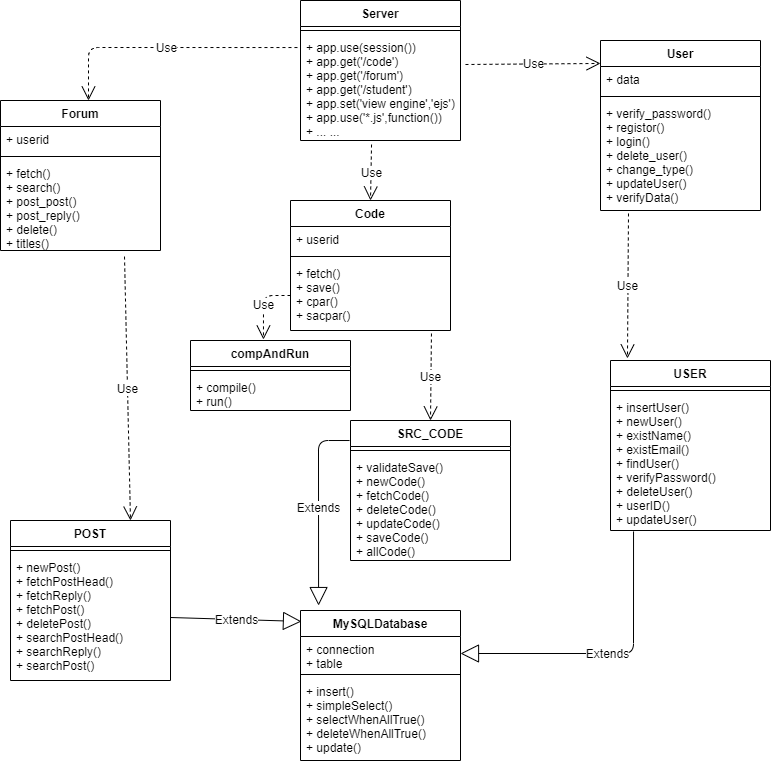
\includegraphics[width=\textwidth]  {Pics/general_class.png}} 
 \label{1}
 \end{figure}
\clearpage

\section{Component-1: Personal Account System}
Personal Account System is a database to provide the identity for student user or teacher user in server and provide several functionalities to user.\newline

\subsection{Use Case Diagram}
\begin{figure}[H]
 \center{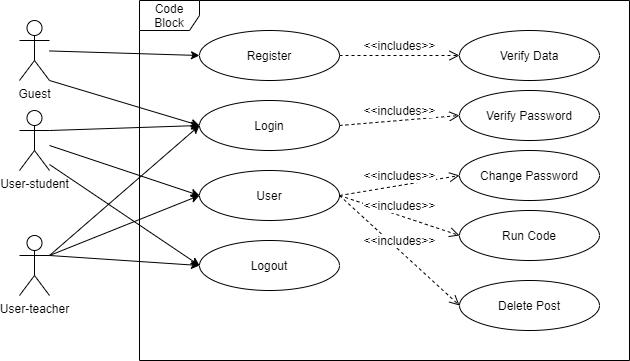
\includegraphics[width=\textwidth]  {Pics/account_use-case.png}}
 \label{2}
 \end{figure}
For a new coming guest, Personal Account System allows he/she can either go to register or login. The register function includes verify data function to verify whether the guest's inputs are all validated. The login function includes verify password function to verify the password input by guest by finding in the database.\newline
For student and teacher user, Personal Account System allows he/she to login and view his/her profile page. The user function provides a page for user to change his/her password, run his/her code and delete his/her post.\newline

\subsection{Sequence Diagram for Guest}
\begin{figure}[H]
 \center{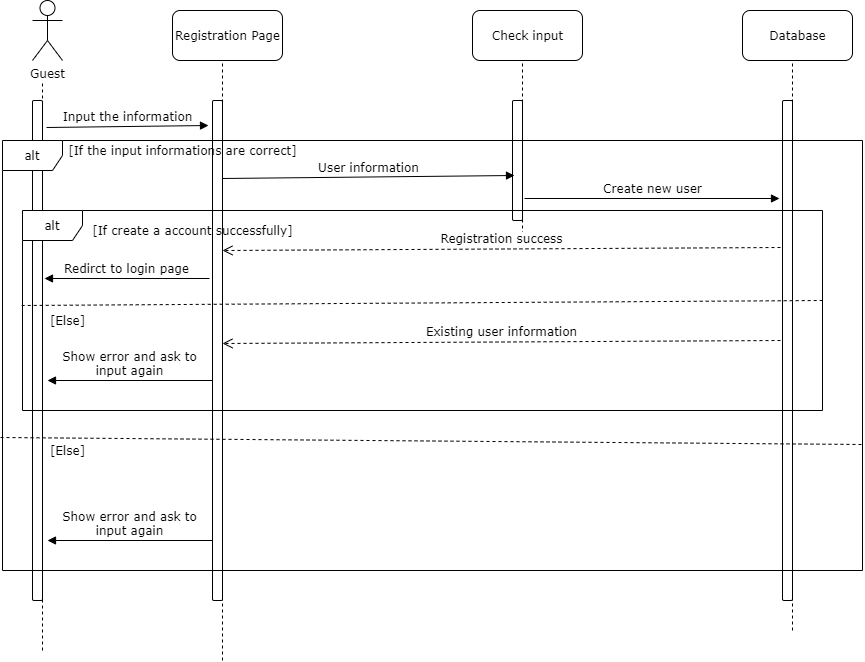
\includegraphics[width=\textwidth]  {Pics/account_sequence_guest.png}} 
 \label{3}
 \end{figure}

\subsection{Activity Diagram for Guest}
\begin{figure}[H]
 \center{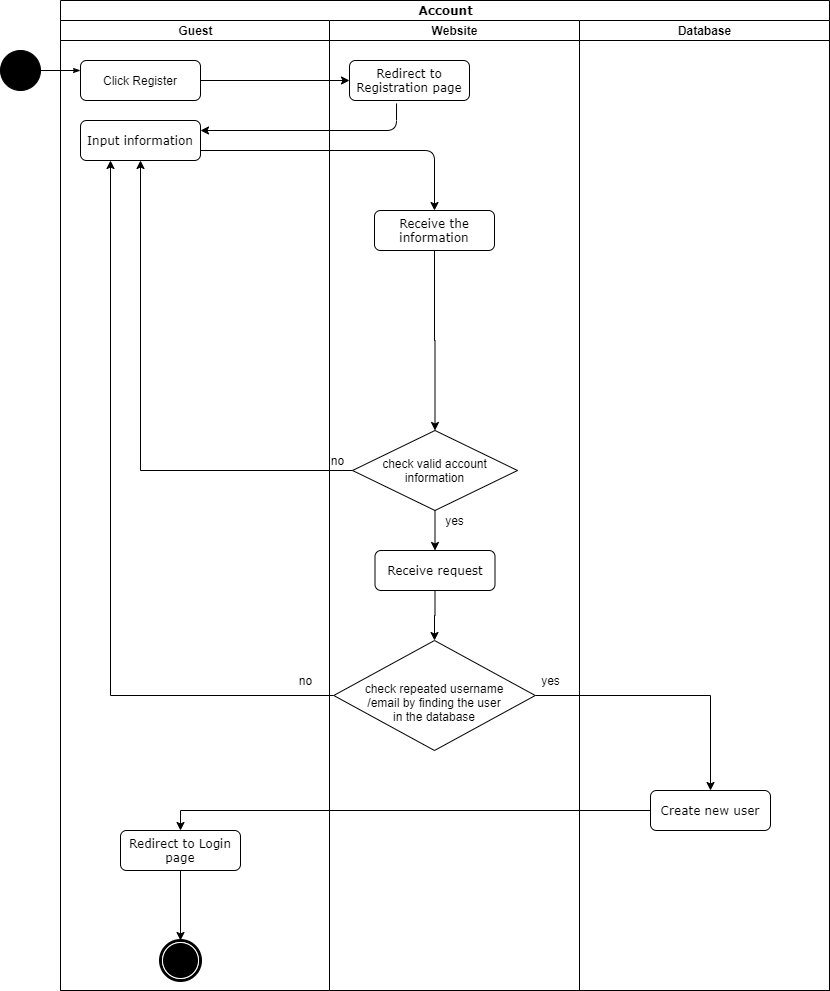
\includegraphics[width=\textwidth]  {Pics/account_activity_guest.png}} 
 \label{4}
 \end{figure}

\subsection{Sequence Diagram for User(login and change password for both types of user)}
\begin{figure}[H]
 \center{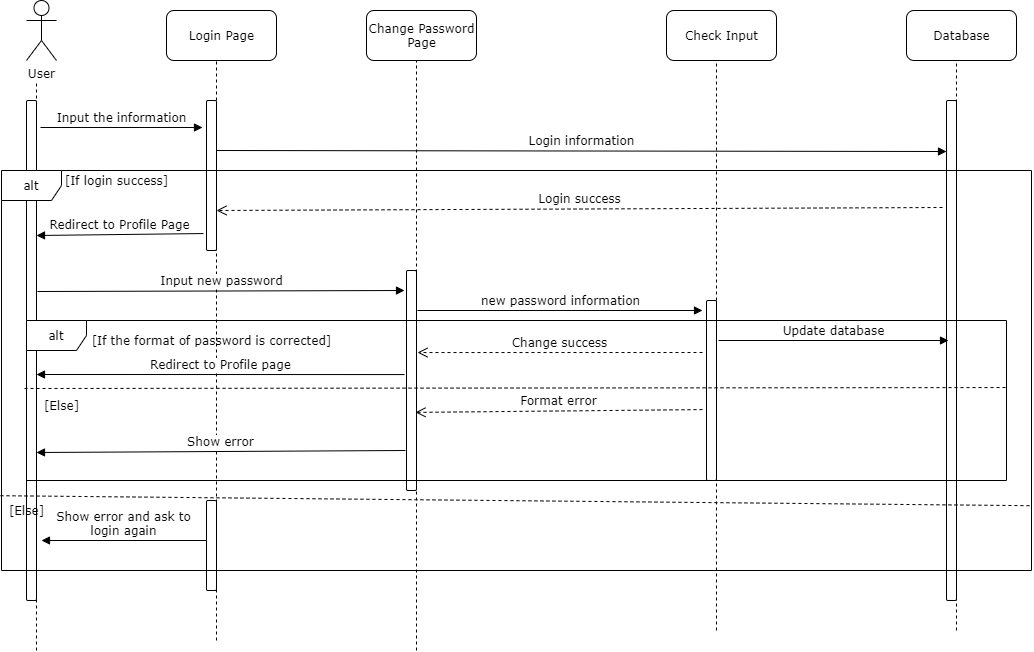
\includegraphics[width=\textwidth]  {Pics/account_sequence_user.png}} 
 \label{10}
 \end{figure}

\subsection{Activity Diagram for User(login and change password for both types of user)}
\begin{figure}[H]
 \center{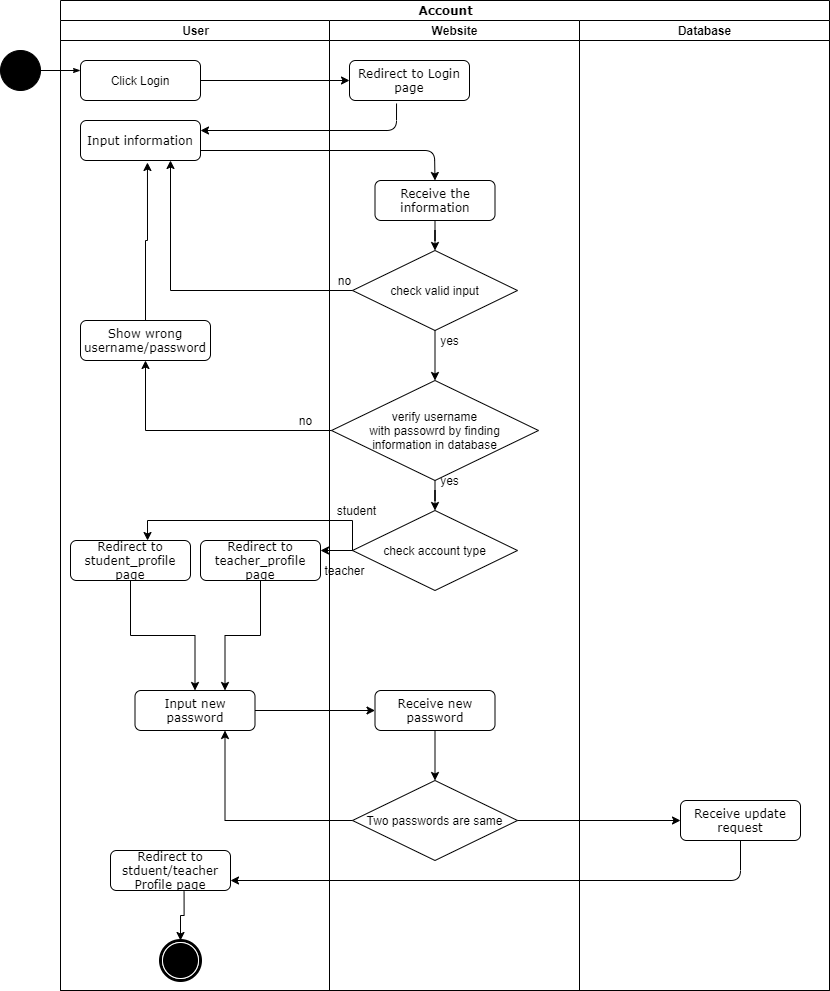
\includegraphics[width=\textwidth]  {Pics/account_activity_user.png}} 
 \label{5}
 \end{figure}

\subsection{Functionality}
This component provided user authentication. It prevented guest without authentication to use some functions which need user identity. For example, writing code, new post and reply. It also provides an easier way for the system to record all the codes, posts and replies that created by that person and user can retrieve those information.\newline

\subsection{Procedures and Functions}
This component provides front-webpages, which are registration page, login page and profile page.\newline\newline
The registration and login page provide basic input checking(format, completion, and length) before passing data request to the server side. After passing the input checking, the webpages will send requests to the database, verifying the data, whether the guest input available username and verifying the password correctness, whether the use login with correct pair of username and password.\newline\newline
The profile page allows users to change their password, run their code and delete their posts. In this page, users can find their profile with username, codes and posts. This page will send a request to server side, getting those information. When user wants to change password, it will do the password verifying for user input, then it will send the request to the server side, changing the password.\newline\newline
For the backend application part, there are lots of functions with SQL statement to retrieve data or update data from the database. It will return the result to the front-webpages after retrieving or updating data, whether it is successful to get or update data.\newline\newline
In conclusion, this system contains the following functions:\newline

\begin{itemize}

\item
\textbf{Registration}
, which is for the guest to register account. This function will verify the data that guest inputs is valid. If the data is valid, create a new account related to the data provided by the guest and redirect to the login page, otherwise, request the guest to input data in correct format.\newline

\item
\textbf{Login}
, which gets the username and password input by user, then verify the correctness from the database. If the input is valid, login to the server, otherwise request the user to input again.\newline

\item
\textbf{Change password}
, which gets the two passwords input by user, then verify whether the two inputs are the same. If the inputs are valid, request server to update the information in database, otherwise request the user to input again.\newline

\item
\textbf{Run code}
, which allow user to choose one of his/her code and redirect to that code page for user to run.

\item
\textbf{Delete Post}
, which allow user to delete the posts wrote by him/her.

\item
\textbf{Logout}
, which stops the access permission with a logged in account.

\end{itemize}
\clearpage

\section{Component-2: Forum}
This is a forum like a system for users to show their codes and discuss on them. The user can write new post, reply to the post, view post and search post.\newline

\subsection{Use Case Diagram}
\begin{figure}[H]
 \center{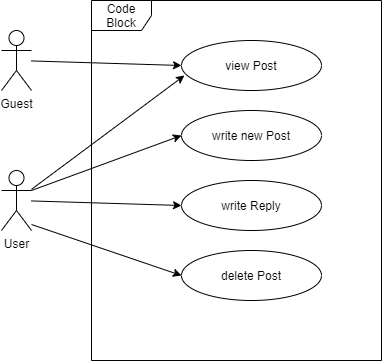
\includegraphics[width=\textwidth]  {Pics/forum_use-case.png}} 
 \label{6}
 \end{figure}
In this system, functions are limited to a guest, guest can only view post and search post. A user is allowed to write new post and write reply. The new post function includes load user code function to list out all the codes that user wrote by finding in the database.\newline

\subsection{Sequence Diagram for Writing new Post and Reply}
\begin{figure}[H]
 \center{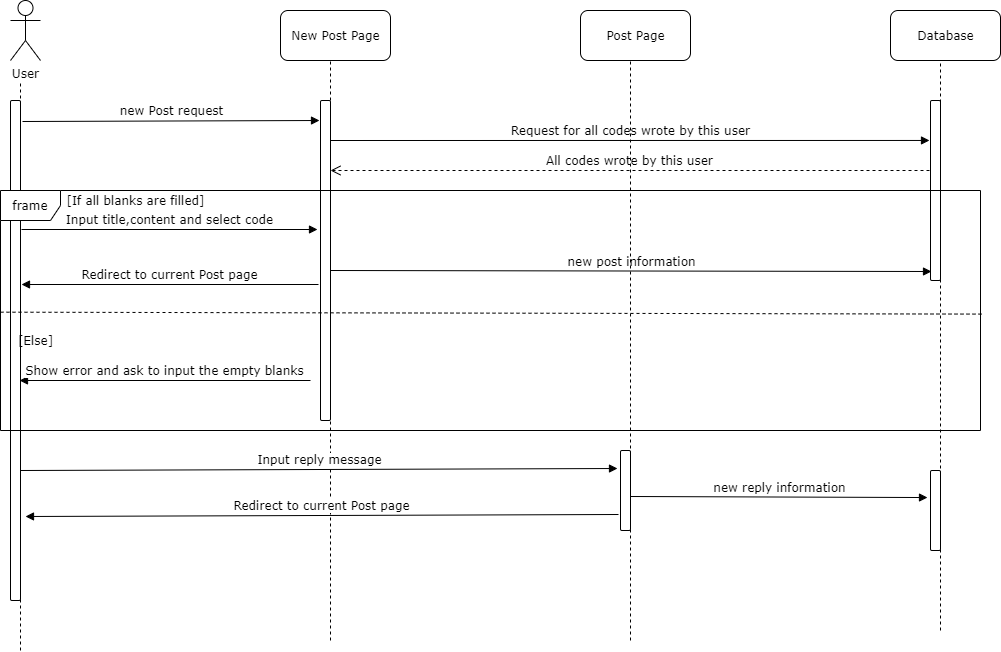
\includegraphics[width=\textwidth]  {Pics/forum_sequence.png}} 
 \label{7}
 \end{figure}

\subsection{Functionality}
The forum component provides a platform for the user to post their code and discuss with other. It contains search post, view post, write new post, write reply functions. Everyone(guest and user)can view post and search post. Only users are allowed to write new post and write reply. If user wants to write a new post but he/she doesn't input title, content and select a code, the page will request user to input all the information, otherwise request the server to update a new post in database.\newline

\subsection{Procedures and Functions}
For the front-end part, the system provided view forum, view post, search post and write new post these 3 pages. For guest, the system will only display view post without reply function, view forum and search post.\newline\newline
In view forum,view post and search post, guests and users are allowed to click inside, viewing the content. When they enter these pages, the server will receive the searching request, and return the required result.\newline\newline
In addition, users are allowed to write new post with the new post page. Users are required to fill in the title, content and select one of their codes in the page. Then the whole data set will be sent to the database, and the server will redirect user to that post page. In a post page, users are allowed to write reply, and the reply will be saved into the database.\newline\newline
In conclusion, this system contains the following functions:

\begin{itemize}

\item
\textbf{View Post}
, which is for everyone(guest and user) to view the post and reply content.\newline

\item
\textbf{Search Post}
, which is a search function receive keyword input by guest or user and return all matching posts.\newline

\item
\textbf{New Post}
, which is for user to write new post with selecting a code and save into the database.\newline

\item
\textbf{Write Reply}
, which is for user to write reply in the post and save into the database.\newline

\end{itemize}
\clearpage

\section{Component-3: Code}
This is a workplace like a online IDE for users to write code in a simple and visualized system.User can drag the block and drop it on the workplace to do coding. The system will automatically generate the code in text format. The user can also save code and run code.\newline

\subsection{Use Case Diagram}
\begin{figure}[H]
 \center{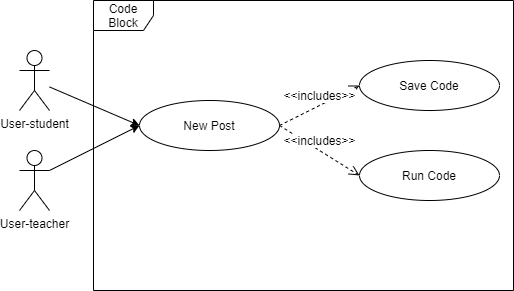
\includegraphics[width=\textwidth]  {Pics/code_use-case.png}} 
 \label{8} 
 \end{figure}
In this system, functions are only provide to user, so guest should register a account first. User is allowed to write code. The write code function includes save code and run code functions.\newline

\subsection{Sequence Diagram for Writing Code, Saving Code and Running Code}
\begin{figure}[H]
 \center{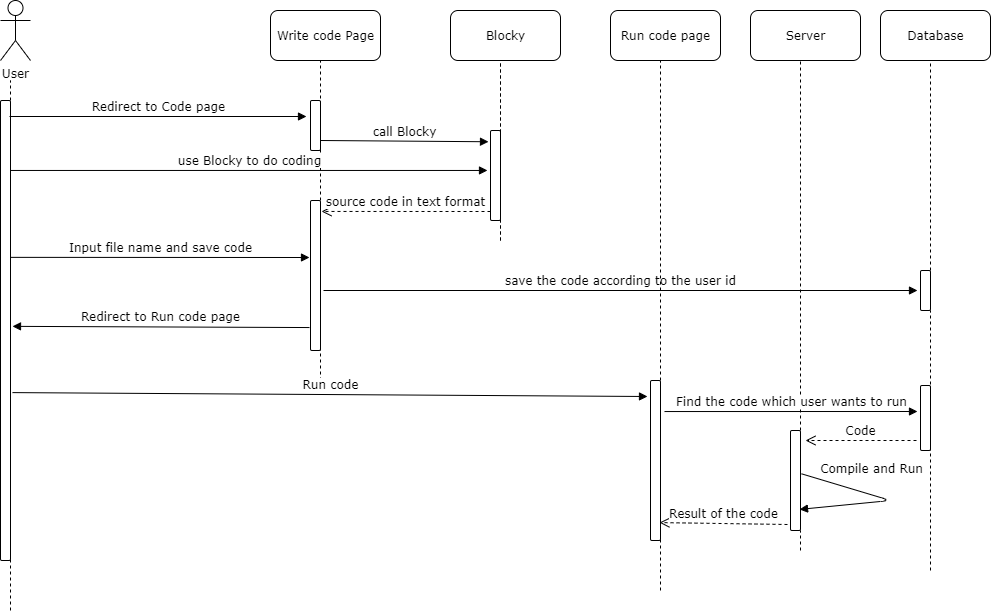
\includegraphics[width=\textwidth]  {Pics/code_sequence.png}} 
 \label{9}
 \end{figure}

\subsection{Functionality}
The code component provides a workplace for the user to do coding online. It contains write code, save code and run code. Only user can use all these functions. 

\subsection{Procedures and Functions}
This component provides front-webpages, which are workplace page, code page and result page.\newline\newline
The workplace page provides a visualized coding area, a code generation area and a form to save code. User should input the file name and copy the code from the code generation area to the form, then the page will send request to server to save the code into the database according to the user identity. After that, the server will redirect the user to that code page.\newline\newline
The code page shows the code wrote by the user for viewing, and there is a input area is used for STDIN when the program required input from keyboard. User can run the code in this page, the page will send the request with the code and input data to server, server will do the compilation and execution. After that, the server will redirect user to result page and return the code result to that page.\newline\newline
For the backend application part, there are lots of functions with SQL statement to retrieve data or update data from the database. Server handles the run code request and return the result to the result page.\newline\newline
In conclusion, this system contains the following functions:\newline

\begin{itemize}

\item
\textbf{Write Code}
, which is for user to do coding in a simple and visualized workplace. User can drag the block and drop it on the workplace and the system generates code in text format.\newline

\item
\textbf{Save Code}
, which is for user to save the code he/she writes. User should input the file name then copy and paste the code generated by the system into the form, then the page sends request to server and ask to update the database according to the user identity. After that, the server redirects user to that code page.

\item
\textbf{Run Code}
, which is for user to run his/her code with optional STDIN input. It sends requests with code and input data to server, server handles the request then do compilation and execution. After that, the server redirects user to result page and return the code result in that page.

\end{itemize}